\documentclass[10pt,conference,compsocconf]{IEEEtran}

\usepackage{hyperref}
\usepackage{fullpage}
\usepackage{times}
\usepackage{fancyhdr,graphicx,amsmath,amssymb}
\usepackage[ruled,vlined]{algorithm2e}
\usepackage{mathtools}
\usepackage{graphicx}	% For figure environment
\usepackage[english]{babel}
\usepackage{comment}

\newtheorem{theorem}{Theorem}
\newtheorem{lemma}[theorem]{Lemma}

\begin{document}
\title{Difference between SGD and random reshuffling}

\author{
  Monde, Diego; Voracek, Vojtech and Wohlleben, Kilian\\
  \textit{Faculty of Computer Science, University of Vienna, Vienna}
}

\maketitle

\begin{abstract}
In this document we will present the difference between stochastic gradient descent and random reshuffling and provide empirical evidence for the latters superiority. 
\end{abstract}

\section{Motivation}
\label{sec:motivation}
\begin{comment}
\begin{theorem}
Differentiable function $f : \mathbb{R}^d \mapsto \mathbb{R}$ is called
\mbox{$\mu$-strongly} convex if the following inequality holds $\forall x, y \in
D(f)$~\cite{StrongConvexity}:

$$
f(y) \geq f(x) + \langle \bigtriangledown f(x), y - x \rangle + {\mu \over
2} || y - x ||^2
$$

\end{theorem}

\begin{theorem}
Differentiable function $f : \mathbb{R}^d \mapsto \mathbb{R}$ is called
\mbox{$L$-Lipschitz}, if there exists a positive constant $L$ such that
$\forall x, y \in D(f)$~\cite{L-Lipschitz}:

$$|| f(x) - f(y) || \leq L ||x - y||$$
\end{theorem}


\begin{theorem}
Differentiable function $f : \mathbb{R}^d \mapsto \mathbb{R}$ is called
\mbox{$L$-smooth} if there exists a positive constant $L$ such that
$\forall x, y \in D(f)$~\cite{L-Lipschitz}:

$$
f(y) \leq f(x) + \langle \bigtriangledown f(x), y - x \rangle + {L \over
2} || y - x ||^2
$$
\end{theorem}

\begin{lemma}
If the gradient of $f$ is \mbox{$L$-Lipschitz}

$$||\bigtriangledown f(x) - \bigtriangledown f(y)|| \leq L ||x-y||,$$

\noindent then is is also \mbox{$L$-smooth}.
\end{lemma}
\end{comment}
\medskip

We consider unconstrained, finite-sum minimization problems or an
empirical risk minimization:

\begin{equation}\label{eq:finite-sum}
\min_{x \in \mathbb{R}} f(x) = \sum_{i = 1}^n f_i(x),
\end{equation}


\noindent where $f$ is a strongly convex function which ensures that there
exists a unique optimal solution whhich is denoted by $x^*$. We also assume
that each individual function $f_i$ is smooth with Lipschitz gradients and
\mbox{$L$-Lipschitz} on a bounded domain. This assumption helps us to make
a particular convergence analysis.
These types of problems are common in many areas of machine learning, one example being Linear Regression.

\medskip

Gradient descent~\cite{GD}:
Traditional approach to minimizing convex functions.

\begin{algorithm}
\SetAlgoLined

  $x:= x_0$ \\
 \For{epochs \texttt{t=1,...,T}}{
    $x_{t+1} := x_t - \alpha \bigtriangledown f(x_t)$
 }
 
 \caption{Gradient descent}
\end{algorithm}
\noindent A initial vector $x_0$, a number of epochs $T$, and
a step size $\alpha$ are defined by the user.

\medskip

Drawback of gradient descent: For large $n$ it is computationally
expensive to evaluate the full gradient.

Instead of GD one can use the Stochastic gradient descent~\cite{SGD} since
$\bigtriangledown f(x) = \sum_{i=1}^n \bigtriangledown f_i(x)$.

\begin{algorithm}
\SetAlgoLined

  $x:= x_0$ \\
 \For{epochs \texttt{t=1, ..., T}}{
    \For{\texttt{i=1, ..., n}}{
      Sample $j \in \{1,..., n\}$ uniformly.
      $x_t^{i+1} := x_t^i - \alpha \bigtriangledown f_j(x_t^i)$
    }
    $x_{t+1} = x_t^n$
 }
 
 \caption{Stochastic gradient descent}
\end{algorithm}

Drawbacks of SGD and also the motivation to introduce Random
reshuffling~\cite{COMPONENTFUNCTION}:

\noindent The specific sample may be chosen more frequently than others. On the
other hand, Random reshuffling guarantees that all samples are selected at
the same frequency.

\medskip

\noindent Random reshuffling:

\noindent In each epoch $t$, we sample indices $[\pi_1, \pi_2,..., \pi_n]$
without replacement from $\{1, 2,..., n\}$, in other words,
$[\pi_1, \pi_2,...\pi_n]$ is a random permutation of the
set $\{1, 2,..., n\}$ and than perform $n$ iterations of the following
form

$$x_t^{i+1} := x_t^i - \alpha \bigtriangledown f_{\pi_i}(x_t^i)$$

\begin{algorithm}
\SetAlgoLined

  $x:= x_0$ \\
 \For{epochs \texttt{t=1, ..., T}}{
    Sample a permutation \\ $[\pi_1, \pi_2,...,\pi_n]$
    of $\{1, 2,...,n\}$ \\
    \For{\texttt{i=1, ..., n}}{
      $x_t^{i+1} := x_t^i - \alpha \bigtriangledown f_{\pi_i}(x_t^i)$
    }
    $x_{t+1} = x_t^{n+1}$
 }
 
 \caption{Random reshuffling}
\end{algorithm}



\section{Optimization problems}

We start with some benchmark functions to analyze the difference between
SGD and RR. Than we used those algorithms to solve a real-life problem.

\subsection{Sphere function}

\noindent Definition~\cite{SPHERE}:
$$f(x) = \sum_{i=1}^n x^2$$
Components of gradient:
$$\bigtriangledown f_i(x) = [0,...,0,2\cdot x_i,0,...,0]$$
Global minimum:
$$f(x^*) = 0$$
$$x^* = [0,...,0]$$
Strong-convexity constant $\mu = 2$, Lipschitz constant \mbox{$L=2$},
number of components of the gradient: $n$. It is presumable one of
the easiest continuous domain optimization problem.

\subsection{The component function}
\noindent Definition~\cite{COMPONENTFUNCTION}:
$$f_1(x) = {1 \over 2}(x-1)^2, f_2(x) = {1 \over 2}(x+1)^2 + {x^2 \over 2}$$
$$f(x) = f_1(x) + f_2(x) = {3 \over 2} x^2 + 1$$
Components of gradient:
$$\bigtriangledown f_1(x) = x - 1, \bigtriangledown f_1(x) = 2x + 1$$
Global minimum:
$$f(x^*) = 1$$
$$x^* = 0$$
Strong-convexity constant $\mu = 3$, Lipschitz constant \mbox{$L=3$},
number of components of the gradient: 2. This is an example of a function where RR is provably better than SGD. \cite{COMPONENTFUNCTION}

\subsection{Inverse Bell Curve}
\noindent Definition~:
$$f(x) = \sum_{i=1}^n 1 - e^{-\frac{x_i^2}{2 \alpha}},$$
Where $\alpha$ is a scaling parameter. 
Components of gradient:
$$\bigtriangledown f_i(x) = \frac{x_i}{\alpha} e^{-\frac{x_i^2}{2 \alpha}}$$
Global minimum:
$$f(x^*) = 0$$
$$x^* = [0,...,0]$$
This is an example of a non-convex function. We want to see, whether SGD and RR behave differently here.

\subsection{Least squares linear regression}

\noindent Definition~\cite{REGRESSION}:
$$f(x) = \sum_{i=1}^n (a_i^T x-b_i)^2 = ||Ax-b||^2,$$
\noindent where $A \in \mathbb{R}^{n \times d}$ and $b \in \mathbb{R}^{n
\times 1}$ are user-specified.
Components of gradient:
$$\bigtriangledown f_i(x) = 2 a_i(a_i^T x - b_i)$$
Global minimum:
$$f(x^*) = ||A (A^T A)^{-1} A^T b - b||$$
$$x^* = (A^T A)^{-1} A^T b$$
Strong-convexity constant $\mu = \lambda_{min}(2A^TA)$, Lipschitz constant
\mbox{$L=\lambda_{max}(2A^TA)$}, where $\lambda_{min}(\cdot),
\lambda_{max}(\cdot)$ denotes the smallest and the largest
eigenvalues. respectively. The number of components of the gradient: $n$.


\section{Experiments}


\medskip

In this work, we use the step size $\alpha = c / (t+1)^s$, where $c>0, s \in
(0, 1]$ for t-th epoch. If we consider q-suffix\footnote{q-suffix
average is obtained by averaging the last $qk$ iterates at iteration
$k$~\cite{COMPONENTFUNCTION}} averages of the iterates for some $q \in (0,1]$
and step size $\alpha = c / (t+1)^s$, one can show that those iterates
of both algorithms (SGD, RR) converge almost surely  at rate
$\mathcal{O}(1 / t^s)$ to the optimal solution~\cite{COMPONENTFUNCTION}.
The specific requirements on the functions $f_i$ decribed in
the~\ref{sec:motivation}~section are necessary to prove this.

We say that the algorithm converged if:

\centerline{$||x - x^{*}|| \leq \epsilon$}

\noindent or alternatively:

\centerline{$||\overline{x}_{q,k} - x^{*}|| \leq \epsilon$}

\noindent for a user-specified $\epsilon$.

\noindent Settings

\begin{itemize}
\item $\epsilon = 10^{-7}$
\item $c = 3$ ($c=50$ for linear regression, $c=30$ for Inverse Bell Curve)
\item $s = 0.9$
\item $q = 0.2$
\item $T = 2000$
\item $x_0 = \sim {\cal U}_{[-10, 10]}^d$
\item $\alpha = 10$
\end{itemize}

The aim of this work is to compare performance of RR and SGD on
specific functions~\ref{eq:finite-sum}. For this purpose, we measured the
performance of those two algorithms on the Sphere function of different
dimensions, on the component function, on the real-world
linear regression - the Diabetes dataset provided by
sklearn~\cite{DIABETES,SKLEARN} and for a self posed non-convex problem. For the diabetes dataset, the dimension
is 10, and the optimized function is a sum of 442 independent functions.

\section{Results}

\begin{figure}[h]
  \centering
  \includegraphics[width=\columnwidth]{sphere_runs}
  \caption{100 runs of SGD and RR on the sphere function of different
  dimensions (2, 3, 5, 10). The bold curve captures the mean over all
  runs of certain algorithm. The graph shows the distance of $x$
  to the optimal solution $x^*$ over epochs.Moreover, the curve
  capturing the convergence rate $\mathcal{O}(1 / k^s)$ is added.}
  \vspace{-3mm}
  \label{fig:sphere1}
\end{figure}

\begin{figure}[h]
  \centering
  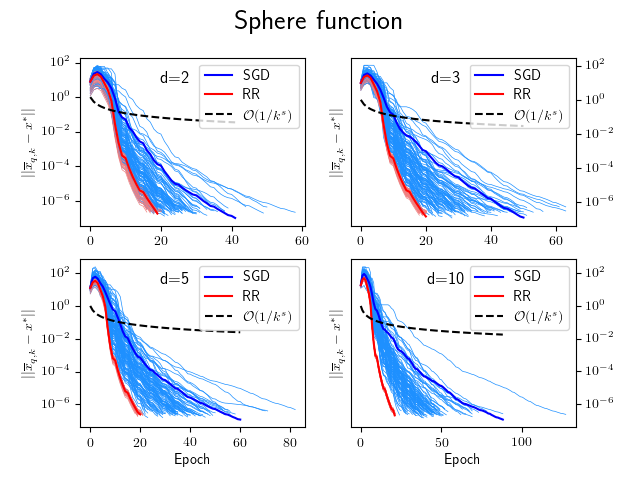
\includegraphics[width=\columnwidth]{Square_runs_average}
  \caption{The graph is similar to~\ref{fig:sphere1}.
  In contrast, this graph shows the distance of q-suffix average
  $\overline{x}_{q,k}$ to the optimal solution $x^*$ over iterations.
  Moreover, the curve capturing the convergence rate
  $\mathcal{O}(1 / k^s)$ is added.}
  \vspace{-3mm}
  \label{fig:squareav1}
\end{figure}

\begin{figure}[h]
  \centering
  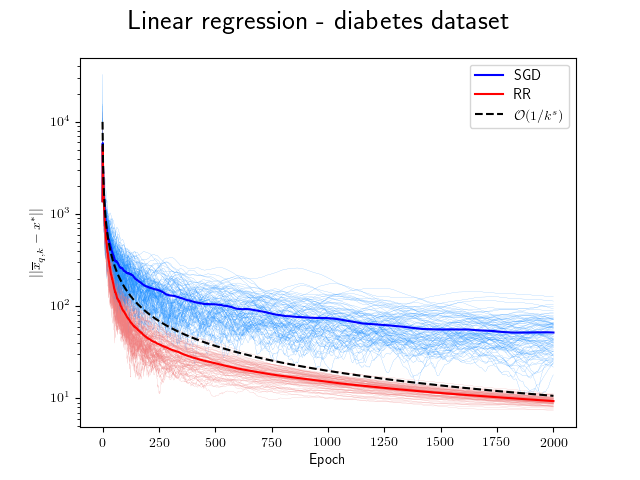
\includegraphics[width=\columnwidth]{LeastSquares_runs_average}
  \caption{100 runs of SGD and RR on the linear regression problem.
   The bold curve captures the mean over all runs of certain algorithm.
   The graph shows the distance of q-suffix average
   $\overline{x}_{q,k}$ to the optimal solution $x^*$ over
   epochs. Moreover, the curve capturing the convergence rate
   $\mathcal{O}(1 / k^s)$ is added.}
  \vspace{-3mm}
  \label{fig:leastsquares1}
\end{figure}

\begin{figure}[h]
  \centering
  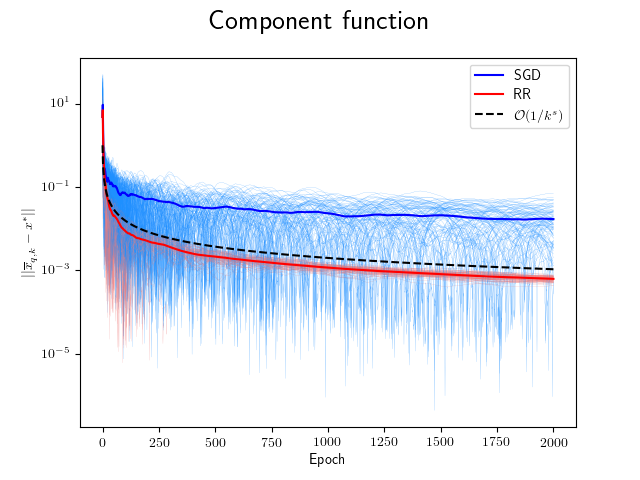
\includegraphics[width=\columnwidth]{ComponentFunction_runs_average}
  \caption{100 runs of SGD and RR on the component function.
   The bold curve captures the mean over all runs of certain algorithm.
   The graph shows the distance of q-suffix average
   $\overline{x}_{q,k}$ to the optimal solution $x^*$ over
   epochs. Moreover, the curve capturing the convergence rate
   $\mathcal{O}(1 / k^s)$ is added.}
  \vspace{-3mm}
  \label{fig:component1}
\end{figure}

\begin{figure}[h]
	\centering
	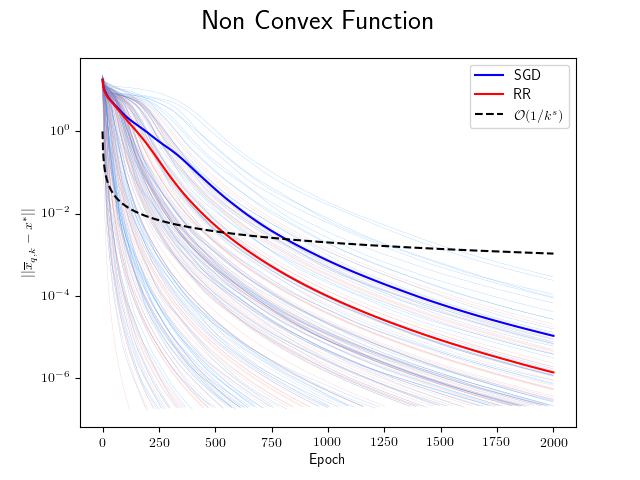
\includegraphics[width=\columnwidth]{Non_Convex_Function_runs_average}
	\caption{100 runs of SGD and RR on the non-convex function.
		The bold curve captures the mean over all runs of certain algorithm.
		The graph shows the distance of q-suffix average
		$\overline{x}_{q,k}$ to the optimal solution $x^*$ over
		epochs. Moreover, the curve capturing the convergence rate
		$\mathcal{O}(1 / k^s)$ is added.}
	\vspace{-3mm}
	\label{fig:nonconvex1}
\end{figure}

\section{Conclusion}

RR has outperformed SGD in all our experiments. We have specifically seen, that RR is much more stable and yields faster convergence. In the case of the sphere function and the inverse bell curve that is due to the fact that all components of $x$ are optimized over equally often, so that no dimension is "neglected". In the case of the component function we could confirm the theoretical superiority of RR proven in \cite{COMPONENTFUNCTION}. For the real world dataset, we have also seen, that optimizing over the entire dataset uniformly is better than leaving the frequency to chance.

\newpage
\bibliographystyle{IEEEtran}
\bibliography{references}

\end{document}
